\documentclass{article}
\usepackage[english]{babel}
\usepackage[utf8x]{inputenc}
\usepackage{amsmath}
\usepackage{graphicx}


\title{12.1 Tests}
\author{chris }
\date{September 2018}

\begin{document}


\noindent BECA / Huson / 12.1 IB Math SL \qquad \qquad Name:\\
3 October 2018
\subsection*{Pre-test: Introduction to differential calculus}
Show working for all problems. State answers exactly or to three significant figures.

\begin{enumerate}

\item Write down the derivative of the function $f(x) = 3x^2 - 3x + 1$.

\item	A function is given as $y = ax^2 + bx + 5$.

\begin{itemize}
    \item[(a)] Find $\displaystyle \frac {dy}{dx}$.
	\item[(b)] If the gradient of this function is 2 when $x$ is 3, write an equation in terms of $a$ and $b$.
	\item[(c)] If the point $(1, -5)$ lies on the graph of the function find a second equation in terms of $a$ and $b$.
\end{itemize}

\item Find $f'(x)$  for the following function. Express your final result without negative exponents:
	 \[	f(x) = \frac{3x^2-x+3}{x}\]

\item	Sketch the function $f(x) = x^2 - 3x - 4$.
\begin{itemize}
    \item[(a)] Find $f(3)$.
	\item[(b)] Find $f'(x)$.
	\item[(c)] What is the slope of a tangent to $f$ when $x=3$?
	\item[(d)] What is the equation of the line tangent to $f$ when $x=3$?
	\item[(e)] What is the equation of the line normal to $f$ when $x=3$?
	\item[(f)] Add the tangent and normal lines to the sketch, labeling the point of tangency.
\end{itemize}

\item Find the equation of the tangent to $\displaystyle f(x) = \frac{1}{2x^2}$ when $x = 2$.

\item Show that the derivative of $f(x)=3x^2-x$ is $f'(x)=6x-1$ from first principles using the definition of the derivative as a limit.

\newpage
\subsection*{Review of function inverses and composition}

\item For the function $f(x) = 2x-7$
\begin{itemize}
    \item[(a)] What is the value of $f(3)$?
	\item[(b)] Solve for $x$ if $f(x)=0$.
	\item[(c)] Find  $f(1-x)$.
	\item[(d)] Find the inverse of $f(x)$,  $f^{-1}(x)$.
\end{itemize}

\item For the function $g(x) = x^2-4$ with $x>0$
\begin{itemize}
    \item[(a)] Simplify the expression $g(x-3)$.
	\item[(b)] Find  $g^{-1}(x)$.
\end{itemize}

\item For the functions $f(x) = 2-x^2$ and $g(x) = 2x-5$
\begin{itemize}
    \item[(a)] What is the value of $g(3)$?
	\item[(b)] Find $(f\circ g)(3)$.
	\item[(c)] Find $(f\circ g)(x)$.
\end{itemize}

\item Find the inverse of $\displaystyle f(x)= \frac {4x-2}{5}$

\item Given that $g(x) = \frac {1}{3} x+2$
\begin{itemize}
    \item[(a)] Find the inverse of $g(x)$.
	\item[(b)] Graph the function $g(x)$ and its inverse on the same axes, using the scale 1 unit equals 1 cm and labeling the graph following IB conventions.
\end{itemize}

\item For the functions defined by $f(x) = 2x$ and $g(x) = x+4$
\begin{itemize}
    \item[(a)] Find an expression for $(f\circ g)(x)$.
	\item[(b)] Find an expression for $(g\circ f)(x)$.
	\item[(c)] Solve $(f\circ g)(x)=(g\circ f)(x)$.
\end{itemize}

\item Write down the domain and range of $f(x)= x^2-6$

\item Using a GDC to analyze the function $\displaystyle f(x)= \frac {3x+2}{x+1}$
\begin{itemize}
    \item[(a)] Write down the equations for the asymptotes.
	\item[(b)] Write down the domain and range of $f(x)$.
\end{itemize}

\newpage
\item Write down the domain and range of the function graphed in Figure \ref{domain}.

\begin{figure}[!ht]
    \centering
    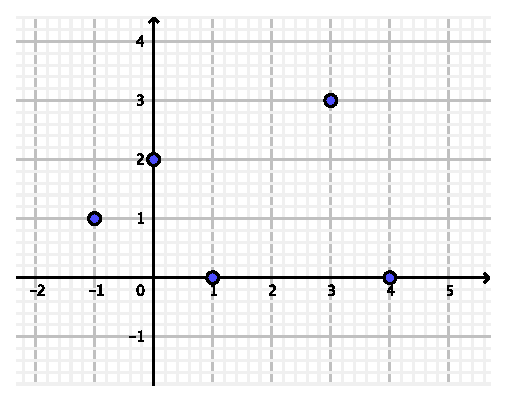
\includegraphics[width=0.6\textwidth]{1-4_domain.eps}
    \caption{Write down domain and range. \label{domain}}
\end{figure}

\item For the function shown in Figure \ref{asymptote}
\begin{figure}[!bh]
    \centering
    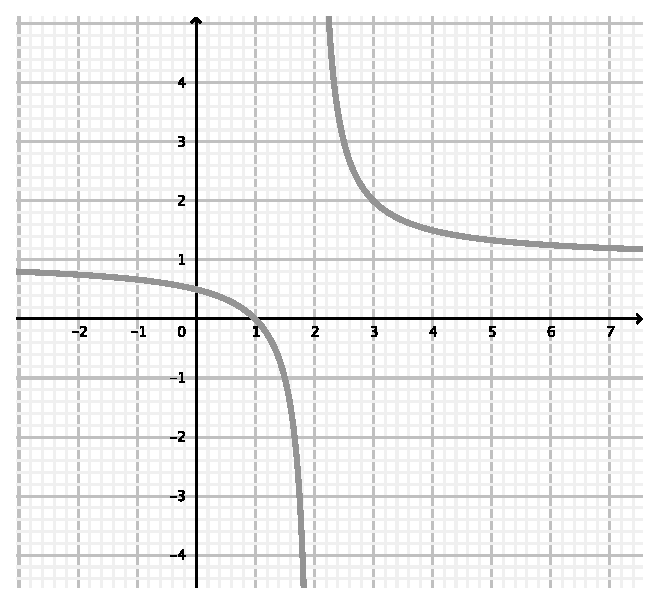
\includegraphics[width=0.7\textwidth]{1-4_asymptotes.eps}
    \caption{Determine asymptotes. \label{asymptote}}
\end{figure}
\begin{itemize}
    \item[(a)] Write down the equations for the asymptotes.
	\item[(b)] Write down the domain and range of the function.
\end{itemize}

\newpage
\noindent BECA / Huson / 11.1 IB Math SL \qquad \qquad Name:\\
20 September 2017\\
Graph accurately in pencil using a straight edge or smooth curve.

\item Given the graph of the function $f(x)$ shown in Figure \ref{inverse}
\begin{itemize}
    \item[(a)] Label points on the function representing $f(-1)=-2$ and $f(4)=-1$
	\item[(b)] Graph the inverse of $f(x)$ on the same axes. Label the inverses of the points named in part (a)
	\item[(c)] Write down the domain and range of $f(x)$.
\end{itemize}
\begin{figure}[!hb]
    \centering
    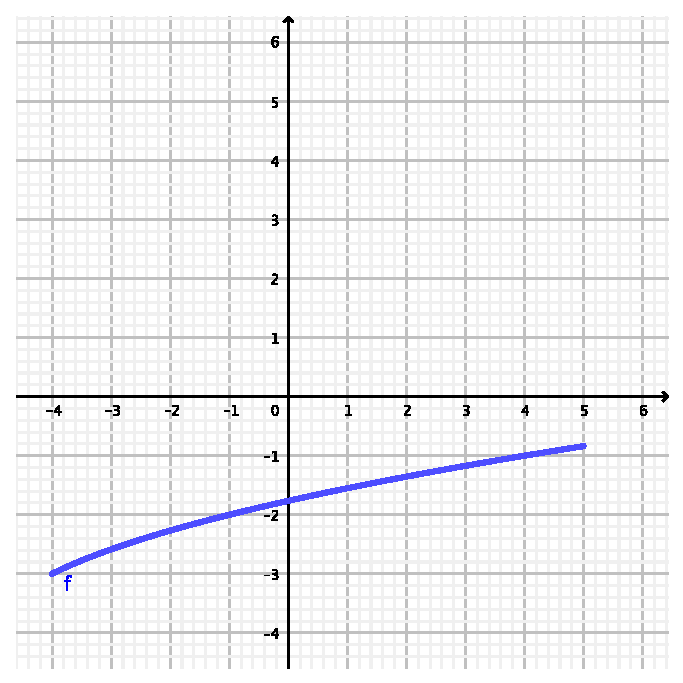
\includegraphics[width=0.75\textwidth]{1-4_inverse.eps}
    \caption{Label given points and plot inverse. \label{inverse}}
\end{figure}

\item Consider the function $f(x) = x^3 - 4x^2 - 3x + 18$.
\begin{itemize}
    \item[(a)] Find the values of $f(x)$ for $a$ and $b$ in the table below:\\
	\begin{tabular}{|l|c|c|c|c|c|c|c|c|c|}
	\hline
	$x$ & -3 & -2 & -1 & 0 & 1 & 2 & 3 & 4 & 5\\
	\hline
    $f(x)$ & -36 & $a$ & 16 & $b$ & 12 & 4 & 0 & 6 & 28\\
	\hline
	\end{tabular}
	\item[(b)] Using a scale of 1 cm for each unit on the $x$-axis and 1 cm for each 5 units on the $y$-axis, draw the graph of $f(x)$ for $-3 \leq x \leq 5$. Label it clearly using IB conventions on the graph paper provided (other side).
\end{itemize}

\end{enumerate}

\end{document}
